\documentclass[a4paper, 11pt]{article}
\usepackage{comment} % enables the use of multi-line comments (\ifx \fi)
\usepackage{fullpage} % changes the margin
\usepackage{url}
\usepackage{graphicx}
\usepackage{caption}
\usepackage{booktabs}

\begin{document}
\noindent
\large\textbf{Deep Learning Course 2017} \hfill \textbf{Ilia Dobrusin} \\
 Autonomous Intelligent Systems \hfill \textbf{Archit Basal} \\
 University Freiburg \hfill Due Date: 18.11.2017

\section*{Deep Learning Lab Course 2017 - Exercise 3}
This exercise has the goal to control an agent on a grid map by feeding the local view of the agent in image form to a neural network which outputs an action on the grid map. First, the training data set is generated from performing A* on the grid map. The training data is then used to train the network.


\section*{Network Architecture}
The network used in this exercise consists of three convolution layers with 32 filters each. After each convolution, max pooling with kernel size 2 and stride 2 is applied. The output of the last max pooling layer is flattened and followed by a fully connected layer. A dropout layer with a dropout rate of 0.5 is used and followed by a fully connected layer. This fully connected layer generated the output vector which specifies the action of the agent on the grid map, using a softmax activation function. The complete architecture can be seen in figure \ref{fig:nn_arch}.

\section*{Experiments and Results}
\subsection*{Baseline}
The first experiment is conducted on a map with dimensions of 28x28 grids with a fixed goal at position (11, 12). The agent has a local view of size 5x5 grid elements and is trained with data consisting of 16500 steps on the grid map. The input consists of a set of images with a history length of 4. The trained network is then evaluated using a validation set. The performance is increased by using bagging with 5 separately trained models, where the output of action of the bagging model during validation is the majority vote on the output action of the 5 models. With bagging the trained models achieved a perfect accuracy of 100\%. Table \ref{tbl:baseline} shows the accuracies of the individual models.

\begin{table}[ht]
	\centering
    \footnotesize
	\begin{tabular}{cl}
		\toprule
		\textbf{Model}	&	\textbf{Accuracy} \\
		\midrule
		1    &	1.0  \\
		2	&	1.0 \\
		3 	&	1.0 \\
        4 	&	1.0 \\
        5 	&	0.9966 \\
		\midrule
        Average 	&	0.9993 \\
		\midrule
        Bagging 	&	1.0 \\
		\bottomrule
    \end{tabular}
    \caption{Accuracies of the individual models for the baseline experiment with a history length of 4 and a local view size of 5x5. }
    \label{tbl:baseline}
\end{table}

\subsection*{Variation of history length and local view size}
\paragraph{History length}
For a history length of 2, the performance dropped slightly compared to the baseline. As shown in table \ref{tbl:hist2} in the left table, the performance of the bagged model is better than the average of the individual models.

For a history length of 8, the performance was better than the performance with history length 2, but the performance suffered due to a mistrained model with a performance of 0.0. The faulty model always performs a single constant action, rendering it useless. This could be caused by neuron death. Since bagging was used, the bagged model still is able to achieve a high accuracy.

\begin{table}[ht]
    \centering
    \footnotesize
        \begin{tabular}[t]{p{2.5cm}c}
            \toprule
            \textbf{Model}	&	\textbf{Accuracy} \\
            \midrule
            1    &	0.9793  \\
            2	&	0.9613 \\
            3 	&	0.9550 \\
            4 	&	0.9776 \\
            5 	&	0.9731 \\
            \midrule
            Average 	&	0.9693 \\
            \midrule
            Bagging 	&	 0.9762\\
            \bottomrule

            % history length = 2
            % - 0.9762 with bagging of 5
            % - 0.9793, 0.9613, 0.9550, 0.9776, 0.9731 (avg=0.9693)
        \end{tabular}
        \begin{tabular}[t]{p{2.5cm}c}
            \toprule
            \textbf{Model}	&	\textbf{Accuracy} \\
            \midrule
            1   &	1.0 \\
            2	&	0.9963 \\
            3 	&	0.9963 \\
            4 	&	0.0 \\
            5 	&	1.0 \\
            \midrule
            Average 	&	0.79044 \\
            \midrule
            Bagging 	&	 0.993127\\
            \bottomrule
            % history length = 8
            % - bagging: 0.993127
            % - 1.0, 0.9963, 0.9559, 0.0, 1.0 (avg=0.79044)
            % 4=Neuron death? always goes up
        \end{tabular}
        \caption{Left: history of 2; Right: history of 8}
        \label{tbl:hist2}
    \end{table}


\paragraph{Local view size}
When reducing the local view to a size of 3x3, the accuracy dropped both for the bagged and individual models. The results for the local view are shown in table \ref{tbl:local_view}. The average of accuracy of the individual models is higher than the accuracy of the bagged model, which indicates that the different models differ in their chosen actions, thus the majority vote used in bagging doesn't necessarily lead to a good action. Since the local view size is reduced, some parts look similar in the local view, making it hard for the network to find the correct action.
For a local view size of 7x7 the trained models achieve a high accuracy, which is not significantly higher than the default local view size of 5x5.

\begin{table}[ht]
    \centering
    \footnotesize
    \begin{tabular}[t]{p{2.5cm}c}
        \toprule
        \textbf{Model}	&	\textbf{Accuracy} \\
        \midrule
        1   &   0.9450 \\
        2	&	0.9234 \\
        3 	&	0.9151 \\
        4 	&	0.9626 \\
        5 	&	0.9954 \\
        \midrule
        Average 	&	0.9483 \\
        \midrule
        Bagging 	&	 0.9118\\
        \bottomrule
    \end{tabular}
    \begin{tabular}[t]{p{2.5cm}c}
        \toprule
        \textbf{Model}	&	\textbf{Accuracy} \\
        \midrule
        1    &	0.9968  \\
        2	&	0.9934 \\
        3 	&	0.9969 \\
        4 	&	1.0 \\
        5 	&	1.0 \\
        \midrule
        Average 	&	0.9974 \\
        \midrule
        Bagging 	&	 1.0\\
        \bottomrule
    \end{tabular}

    \caption{Left table: local view size of 3x3 - Right: local view of size 7x7; }
    \label{tbl:local_view}
\end{table}

\subsection*{Variation of target location and map}
This experiment should show how well the trained network generalizes on different target locations and unseen maps. When changing the target location on the training map, the agent tries to move to the trained target coordinates without actively searching for the target. Regardless of the new target location the agent moves around the trained target location.\\
In order to test the model on a different map, the original map was flipped along the X and Y axes respectively to generate two new experimental maps. The target location was mapped accordingly, such that even though the target was still placed at the same location on the map as the training map and target, the coordinates changed. On an unseen map the agent is not able to perform any meaningful movements, as the model can not account for the changed context. The agent tries to approach the same coordinates as the old map on which it was trained, but since it relies on a memory of "corridors" to generate the appropriate actions, it results in meaningless actions that are no better than random movements, if not worse.

% - The agent tries to go to the old (trained) target coordinates but is not actually searching for the target.
% -  Regardless of the new target location the agent moves around the old target location
% - accuracy of 0.1 (randomly reached target)
% What happens if you change the map after training (how well does your agent generalize) ?
% - Does not generalize at all, the  agent is not able to perform meaningful movements in the new context.


\section*{Evaluation}
Generalization of agent across target locations and maps
The performance of the trained models is good as long as the map and target location stay fixed. In order to generalize better across different maps and target locations the following methods could be useful.  \\
In order to increase performance and reduce overfitting, bagging can be used. This was tested out in the experiments, but resulted in poor performance for the generalized experiment, where the performance of the bagged model was equally bad compared to the individual models. The bagged approach can still be useful when applied to the following improvements.  \\
In addition to the history of previous steps, some additional information of the map can increase performance of the model. This additional map information could consist of a general direction or aerial distance to the target. A local view of the target area could also increase performance, as the model could infer information from it.  \\
Also, random exploration can be added to the network output, which could help to resolve situation in which the agent is stuck in an area of the map.


% - Expansion: dynamic environment (moving object, agents... + different types of object)

\begin{figure}[ht]
    \centering
    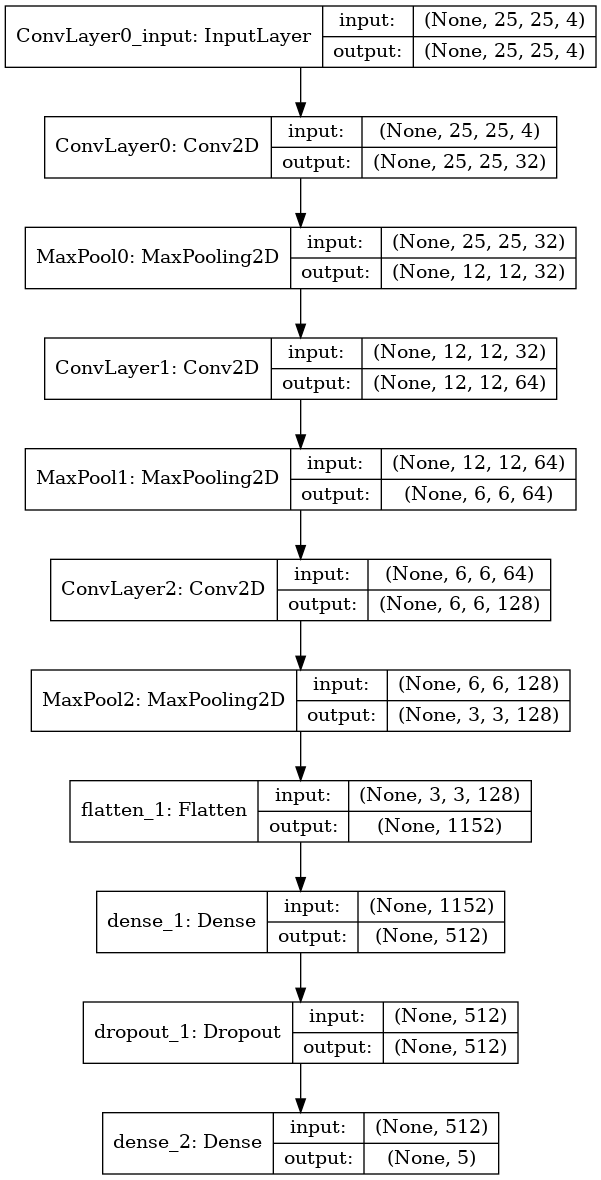
\includegraphics[height=12cm]{images/architecture.png}
        \caption{The architecture of the neural network used in this exercise}
        \label{fig:nn_arch}
\end{figure}

\end{document}
